\documentclass[11pt,aspectratio=169]{beamer}
\usetheme{Madrid}
\usecolortheme{default}

% ── Color Palette (matching HUST DS theme) ────────────────────────────────────
\definecolor{primary}{RGB}{192,33,53}       % Plum Red
\definecolor{secondary}{RGB}{0,128,128}     % Teal
\definecolor{accent}{RGB}{227,114,34}       % Orange accent
\definecolor{lightbg}{RGB}{245,248,252}     % Light background
\definecolor{codebg}{RGB}{30,30,30}
\definecolor{codegreen}{RGB}{80,200,120}
\definecolor{codeyellow}{RGB}{220,180,80}
\definecolor{neutral}{RGB}{110,110,110}
\definecolor{navy}{HTML}{1a2744}
\definecolor{crimson}{HTML}{A32D2D}
\definecolor{teal}{HTML}{0F6E56}
\definecolor{NodeBlue}{RGB}{135,206,235}
\definecolor{NodeGreen}{RGB}{144,238,144}
\definecolor{NodeOrange}{RGB}{255,200,100}
\definecolor{NodePurple}{RGB}{206,170,206}

\setbeamercolor{palette primary}{bg=primary,fg=white}
\setbeamercolor{palette secondary}{bg=primary!80,fg=white}
\setbeamercolor{palette tertiary}{bg=primary!60,fg=white}
\setbeamercolor{palette quaternary}{bg=primary,fg=white}
\setbeamercolor{structure}{fg=primary}
\setbeamercolor{section in toc}{fg=primary}
\setbeamercolor{block title}{bg=neutral,fg=white}
\setbeamercolor{block body}{bg=lightbg}
\setbeamercolor{block title example}{bg=secondary,fg=white}
\setbeamercolor{block body example}{bg=secondary!10}
\setbeamercolor{block title alerted}{bg=accent,fg=white}
\setbeamercolor{block body alerted}{bg=accent!10}
\setbeamercolor{alerted text}{fg=accent}

% ── Packages ──────────────────────────────────────────────────────────────────
\usepackage[utf8]{inputenc}
\usepackage[T1]{fontenc}
\usepackage[english]{babel}
\usepackage{amsmath,amssymb,amsfonts}
\usepackage{graphicx}
\usepackage{booktabs}
\usepackage{array}
\usepackage{colortbl}
\usepackage{tabularx}
\usepackage{xcolor}
\usepackage{tikz}
\usetikzlibrary{shapes.geometric,shapes.misc,arrows.meta,positioning,fit,backgrounds,calc}
\usepackage{hyperref}
\usepackage{multirow}
\usepackage{multicol}

\graphicspath{{figures/}{img/}}

% ── Beamer settings ───────────────────────────────────────────────────────────
\setbeamercovered{transparent=20}
\setbeamertemplate{navigation symbols}{}
\setbeamertemplate{footline}[frame number]
\setbeamertemplate{itemize items}[circle]
\setbeamertemplate{enumerate items}[default]
\setbeamertemplate{frametitle}{
    \nointerlineskip
    \begin{beamercolorbox}[sep=0.5cm,wd=\paperwidth]{frametitle}
        \vbox{}\vskip-2ex%
        \strut\insertframetitle\strut
        \hfill
        \IfFileExists{img/logo-dhbk.png}{\includegraphics[height=0.8cm]{img/logo-dhbk.png}}{}
        \vskip-1.5ex
    \end{beamercolorbox}
}
\setbeamerfont{block body}{size=\small}
\setbeamerfont{frametitle}{size=\normalsize,series=\bfseries}

% ══ Custom storytelling macros ═════════════════════════════════════════════════
% Objective + Technique banner for follow-up investigation slides
\newcommand{\aimtech}[2]{%
  \begin{beamercolorbox}[wd=\textwidth,sep=5pt,rounded=true]{palette secondary}
    \footnotesize\textbf{Objective:}~#1\\[1pt]\textbf{Technique:}~#2
  \end{beamercolorbox}\vspace{3pt}%
}
% Right-column insight block
\newenvironment{insights}{%
  \begin{block}{\small\textbf{Insights \& observations}}\footnotesize}{%
  \end{block}}
% Small "so-what" strip at slide bottom
\newcommand{\sowhat}[1]{%
  \vspace{2pt}\begin{beamercolorbox}[wd=\textwidth,sep=4pt,rounded=true]{block title alerted}%
  \footnotesize\textbf{So what:}~#1\end{beamercolorbox}}

% Process-strip node style
\tikzset{
  pstep/.style={rectangle, rounded corners=2pt, draw=primary!60, fill=lightbg,
    text=navy, font=\scriptsize, align=center, minimum height=0.9cm,
    inner sep=3pt, text width=1.9cm},
  parrow/.style={-{Stealth[length=2mm]}, primary!70, thick}
}

% ── Title Information ─────────────────────────────────────────────────────────
\title[Churn Prediction \& Segmentation]{Customer Churn Prediction \& Segmentation for a Digital Bank}
\subtitle{From Business Understanding to a Leakage-Safe, Budget-Aware Retention Pipeline}
\author{
    Author 1$^1$ \and Author 2$^2$ \and Author 3$^1$ \\
    \small{
        \href{mailto:author1@email.com}{\texttt{author1@email.com}} \and
        \href{mailto:author2@email.com}{\texttt{author2@email.com}} \and
        \href{mailto:author3@email.com}{\texttt{author3@email.com}}
    }
    \\
    Author 4$^4$ \and Author 5$^5$ \\
    \small{
        \href{mailto:author1@email.com}{\texttt{author1@email.com}} \and
        \href{mailto:author2@email.com}{\texttt{author2@email.com}}
    }
}

\institute[SOICT]{
  Master of Data Science Program, \\
  School of Information and Communications Technology, \\
  Hanoi University of Science and Technology
}
\date{July 2026}

% ══════════════════════════════════════════════════════════════════════════════
\begin{document}

% ── SLIDE 1: TITLE ────────────────────────────────────────────────────────────
\begin{frame}[plain,noframenumbering]
  \titlepage
\end{frame}

% ── SLIDE 2: TABLE OF CONTENTS ────────────────────────────────────────────────
\begin{frame}{Table of Contents}
  \tableofcontents[hideallsubsections]
\end{frame}

% ═════════════════════════════════════════════════════════════════════════════
\section{Project Overview}
% ═════════════════════════════════════════════════════════════════════════════

% ── One-in-five framing + CRISP-DM process ────────────────────────────────────
\begin{frame}{One in five customers has already left --- the goal is the recoverable 10\%}
  \begin{columns}[T]
    \begin{column}{0.36\textwidth}
      \centering
      \begin{beamercolorbox}[wd=\textwidth,sep=8pt,rounded=true]{block title alerted}
        \centering{\Huge\textbf{20.37\%}}\\[2pt]{\footnotesize churn rate (\(\approx\)1:4)}
      \end{beamercolorbox}\vspace{6pt}
      \begin{beamercolorbox}[wd=\textwidth,sep=8pt,rounded=true]{block title example}
        \centering{\Huge\textbf{10,000}}\\[2pt]{\footnotesize customers, 12 real columns}
      \end{beamercolorbox}\vspace{6pt}
      \footnotesize\textit{``Which customers are likely to churn next quarter, and in which segment --- so retention is targeted, not sprayed?''}
    \end{column}
    \begin{column}{0.62\textwidth}
      \small\textbf{CRISP-DM pipeline followed end to end:}\\[8pt]
      \begin{center}
      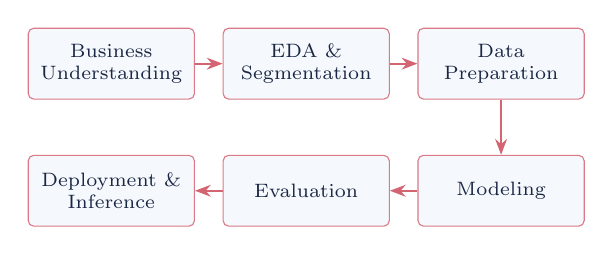
\begin{tikzpicture}[node distance=0.35cm]
        \node[pstep] (a) {Business\\Understanding};
        \node[pstep, right=of a] (b) {EDA \&\\Segmentation};
        \node[pstep, right=of b] (c) {Data\\Preparation};
        \node[pstep, below=0.7cm of c] (d) {Modeling};
        \node[pstep, left=of d] (e) {Evaluation};
        \node[pstep, left=of e] (f) {Deployment \&\\Inference};
        \draw[parrow] (a)--(b); \draw[parrow] (b)--(c);
        \draw[parrow] (c)--(d); \draw[parrow] (d)--(e); \draw[parrow] (e)--(f);
      \end{tikzpicture}
      \end{center}
      \vspace{2pt}
      \sowhat{Every downstream decision is train-only and leakage-audited --- rigor is the product, not just the AUC.}
    \end{column}
  \end{columns}
\end{frame}

% ── Three questions → three approaches + guardrail ─────────────────────────────
\begin{frame}{Three business questions map to three analytical approaches}
  \aimtech{Frame the ask before modeling --- avoid the top cause of wasted DS effort.}%
          {Question-to-technique mapping (Descriptive / Predictive / Prescriptive).}
  \renewcommand{\arraystretch}{1.3}
  \begin{center}
  \footnotesize
  \begin{tabularx}{\textwidth}{@{}p{0.30\textwidth}p{0.22\textwidth}X@{}}
    \toprule
    \textbf{Question} & \textbf{Approach} & \textbf{Method} \\
    \midrule
    Q1 --- \emph{Who} is likely to churn? & Classification & Logistic baseline \(\to\) tree ensembles \(\to\) soft voting; budget-K operating point \\
    Q2 --- \emph{Which segment}? & Descriptive / Diagnostic & 4 RFM-proxy segments + \texttt{age\_band}\(\times\)\texttt{products} heatmap + K-means cross-check \\
    Q3 --- \emph{How} to target retention? & Prescriptive & Precision@K vs.\ retention budget; expected value; A/B test to prove causality \\
    \bottomrule
  \end{tabularx}
  \end{center}
  \begin{alertblock}{\small Governance guardrail --- two-layer conclusion rule}
    \footnotesize Behavioral data is \textbf{synthetic} (generated \emph{conditionally on} churn). It proves only that the \textbf{pipeline is correct}. All \textbf{business} conclusions are drawn from the 12 \textbf{real} columns only.
  \end{alertblock}
\end{frame}

% ═════════════════════════════════════════════════════════════════════════════
\section{Exploratory Data Analysis}
% ═════════════════════════════════════════════════════════════════════════════

% ── EDA opener: 6-step read + data quality ────────────────────────────────────
\begin{frame}{Clean data, one dominant driver: a six-pass read of 10,000 customers}
  \aimtech{Turn a raw table into a defensible ``what drives churn'' summary.}%
          {Six-step EDA: attributes \(\to\) univariate \(\to\) bivariate \(\to\) multivariate \(\to\) anomalies \(\to\) features.}
  \begin{columns}[T]
    \begin{column}{0.55\textwidth}
      \centering
      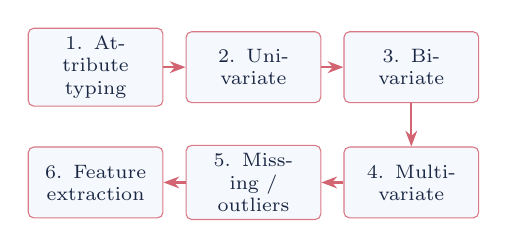
\begin{tikzpicture}[node distance=0.28cm]
        \node[pstep,text width=1.5cm] (s1) {1. Attribute\\typing};
        \node[pstep,text width=1.5cm,right=of s1] (s2) {2. Uni-\\variate};
        \node[pstep,text width=1.5cm,right=of s2] (s3) {3. Bi-\\variate};
        \node[pstep,text width=1.5cm,below=0.55cm of s3] (s4) {4. Multi-\\variate};
        \node[pstep,text width=1.5cm,left=of s4] (s5) {5. Missing /\\outliers};
        \node[pstep,text width=1.5cm,left=of s5] (s6) {6. Feature\\extraction};
        \draw[parrow](s1)--(s2);\draw[parrow](s2)--(s3);\draw[parrow](s3)--(s4);
        \draw[parrow](s4)--(s5);\draw[parrow](s5)--(s6);
      \end{tikzpicture}\\[4pt]
      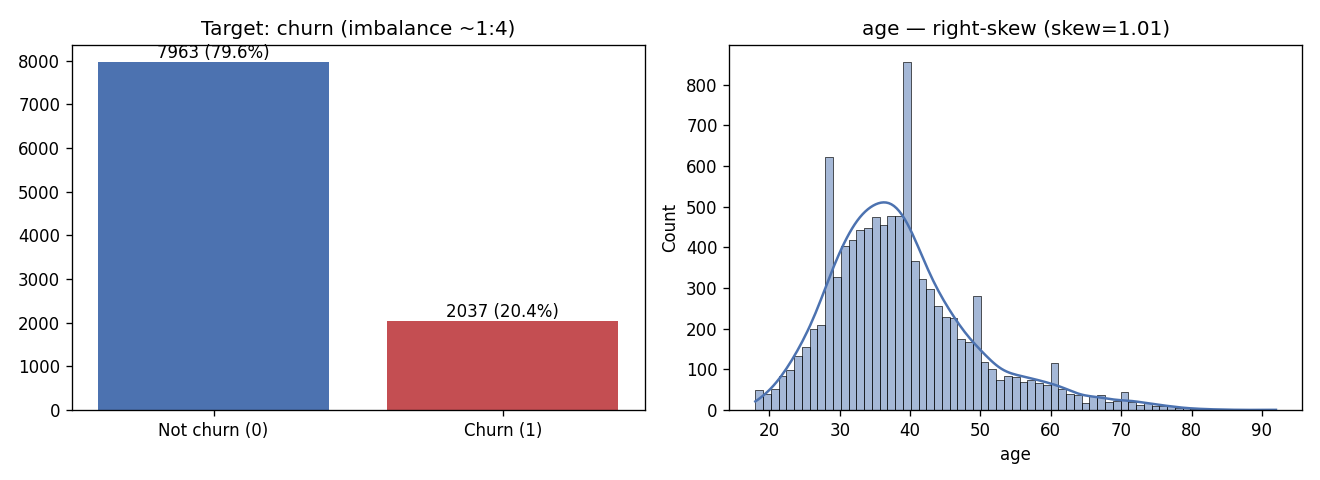
\includegraphics[width=0.98\linewidth]{target_and_age_v2.png}
    \end{column}
    \begin{column}{0.45\textwidth}
      \begin{insights}
        \begin{itemize}
          \item Quality is clean: \textbf{0 duplicates, 0 missing}; only \texttt{age} is right-skewed (\(\approx\)1.0).
          \item Class imbalance confirmed: \textbf{20.37\%} churn \(\to\) carried to \texttt{class\_weight}/SMOTE.
          \item \texttt{age} shows a \textbf{non-linear} churn relationship (peaks mid-life) --- flagged for remediation.
          \item No numeric pair exceeds \(|r|>0.5\) \(\to\) no worrying collinearity.
        \end{itemize}
      \end{insights}
    \end{column}
  \end{columns}
\end{frame}

% ── EDA: churn drivers effect size ────────────────────────────────────────────
\begin{frame}{Product holdings --- not demographics --- dominate churn risk}
  \aimtech{Rank churn drivers on the real columns to focus modeling and retention.}%
          {Effect sizes: Cramér's V (categorical), \(\eta^2\) (numeric); \(\chi^2\)/ANOVA significance.}
  \begin{columns}[T]
    \begin{column}{0.55\textwidth}
      \centering
      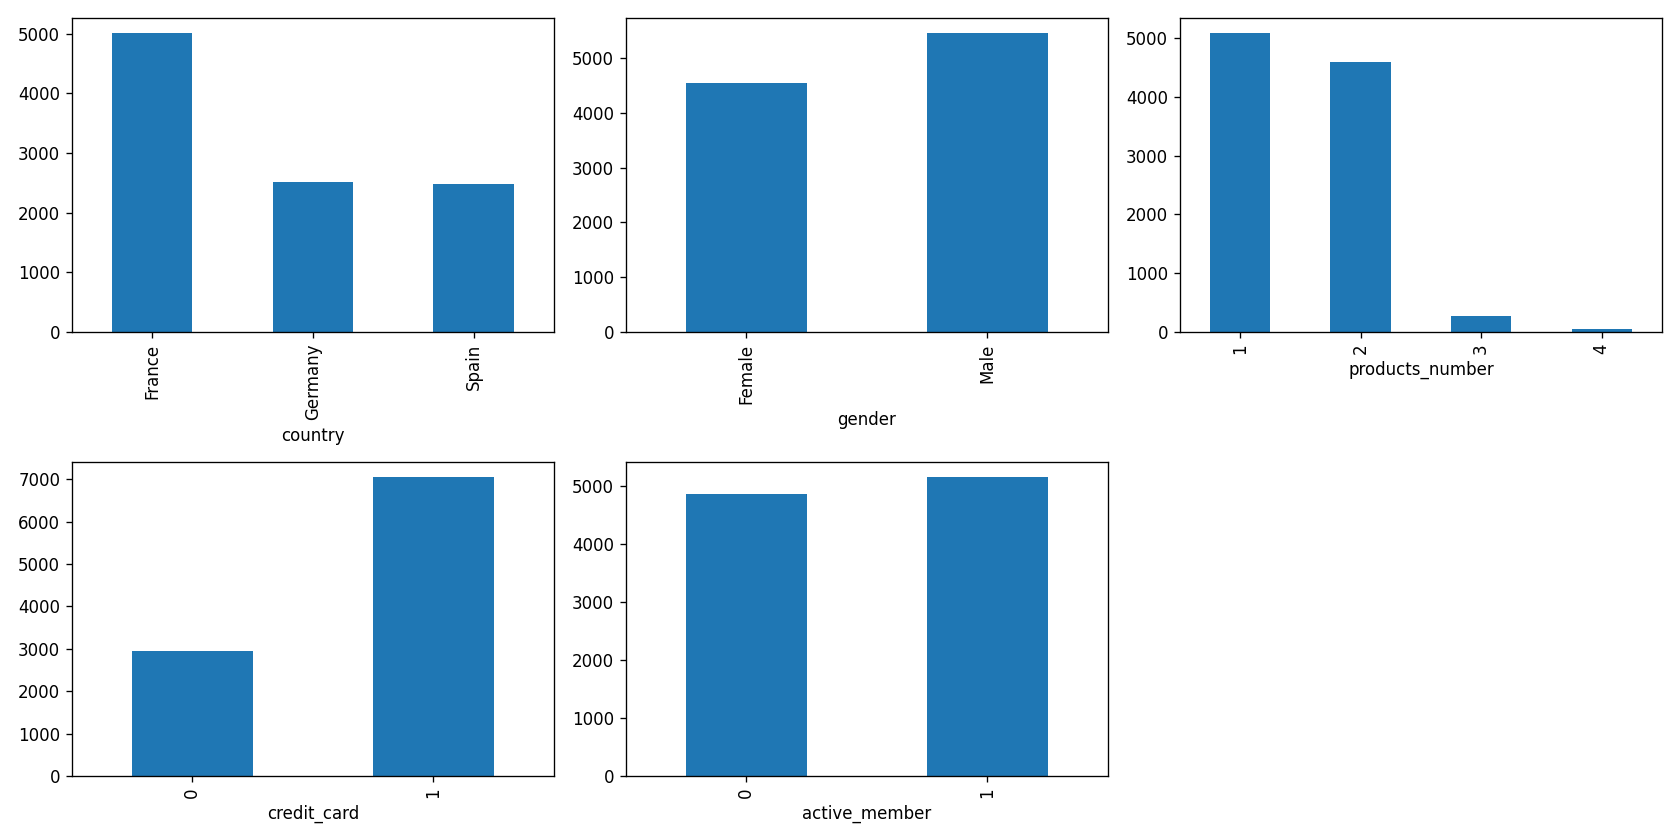
\includegraphics[height=0.66\textheight]{univariate_categorical.png}
    \end{column}
    \begin{column}{0.45\textwidth}
      \begin{insights}
        Effect-size ranking (real data):
        \begin{itemize}
          \item \texttt{products\_number} \textbf{V=0.388} \(\gg\) rest
          \item \texttt{country} 0.174 \(>\) \texttt{active\_member} 0.156 \(>\) \texttt{gender} 0.106
          \item \texttt{age} \(\eta^2\)=0.081 (non-linear)
          \item \texttt{tenure}, \texttt{salary}, \texttt{credit\_card} \(\approx\)\textbf{0} --- not significant
        \end{itemize}
        \textit{The ``new customers churn more'' hypothesis is \textbf{not} supported (\texttt{tenure} \(\eta^2\!\approx\!0\)).}
      \end{insights}
      \sowhat{A product-count rule can flag risk with \emph{no model at all}.}
    \end{column}
  \end{columns}
\end{frame}

% ── EDA: interaction heatmap ──────────────────────────────────────────────────
\begin{frame}{Products \(\geq\)3 push churn toward 100\%; risk peaks at ages 50--59}
  \aimtech{Expose the interaction the univariate view hides.}%
          {Churn-rate pivot heatmap over \texttt{age\_band} \(\times\) \texttt{products\_number}.}
  \begin{columns}[T]
    \begin{column}{0.58\textwidth}
      \centering
      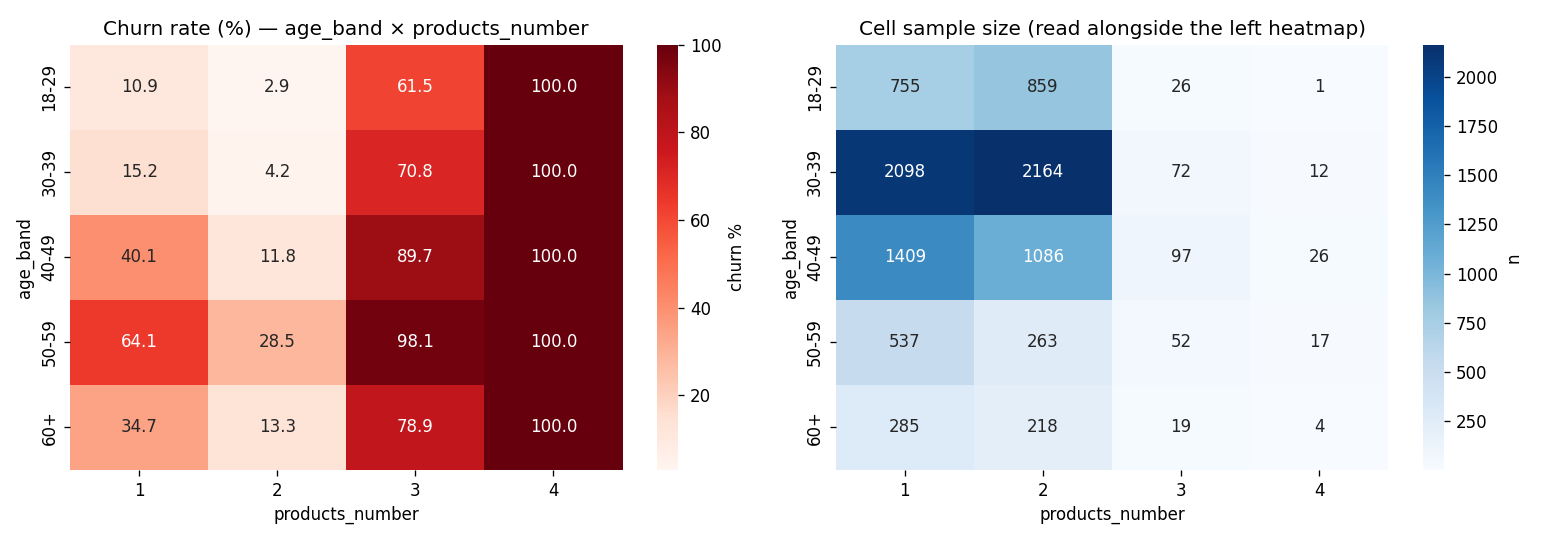
\includegraphics[width=0.99\linewidth]{churn_heatmap_age_products_v2.png}
    \end{column}
    \begin{column}{0.42\textwidth}
      \begin{insights}
        \begin{itemize}
          \item \texttt{products=4} \(\to\) \textbf{100\%} churn; \texttt{products=3} \(\to\) \textbf{82.7\%} (small \(n\): trust direction, wide CIs).
          \item Churn is \textbf{non-monotone} in age, peaking at \textbf{56\%} for the 50--59 band.
          \item The two effects \textbf{compound}: inactive, multi-product, mid-life = the darkest cells.
        \end{itemize}
      \end{insights}
      \sowhat{These cells define the At-Risk list before any classifier runs.}
    \end{column}
  \end{columns}
\end{frame}

% ── EDA: segmentation Q2 ──────────────────────────────────────────────────────
\begin{frame}{Four rule-based segments split risk 13\(\times\): At Risk 70\% vs.\ Champion 5.4\%}
  \aimtech{Answer Q2 --- assign every customer to an actionable group on real columns.}%
          {Priority-ordered RFM-proxy rules (\texttt{products}, \texttt{tenure}, \texttt{active}, \texttt{age}); K-means cross-check.}
  \begin{columns}[T]
    \begin{column}{0.55\textwidth}
      \centering
      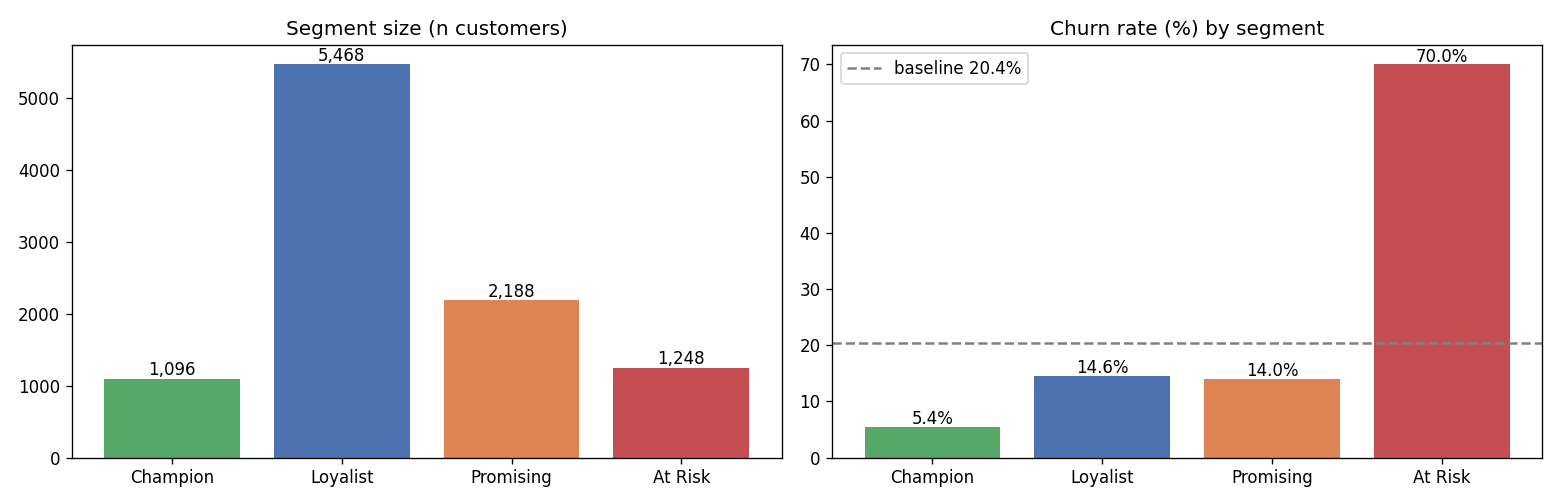
\includegraphics[height=0.34\textheight]{segment_size_churn_v2.png}\\[2pt]
      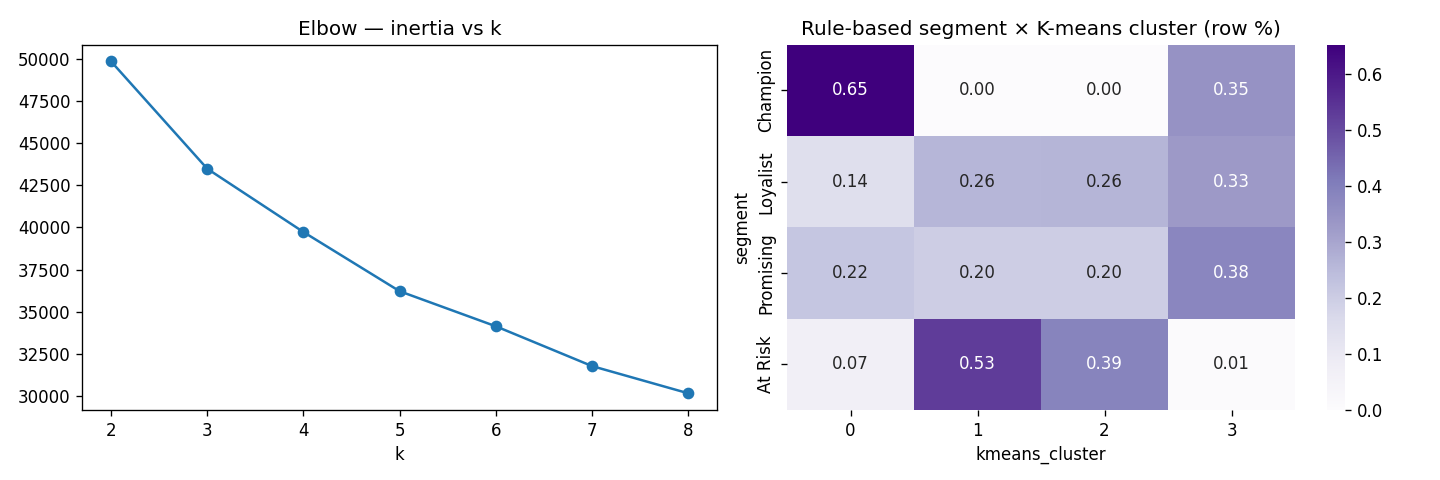
\includegraphics[height=0.28\textheight]{segment_vs_kmeans_v2.png}
    \end{column}
    \begin{column}{0.45\textwidth}
      \begin{insights}
        \begin{itemize}
          \item \textbf{At Risk} --- \(n\)=1{,}248, \textbf{70\%} churn (products\(\geq\)3 or inactive 45+).
          \item \textbf{Champion} --- \(n\)=1{,}096, \textbf{5.4\%} churn (active, tenure\(\geq\)6, 2 products).
          \item \textbf{Promising} (new, tenure\(\leq\)2) and \textbf{Loyalist} (rest) fill the middle.
          \item K-means (silhouette 0.25) recovers the same structure \(\to\) rules aren't missing natural clusters.
        \end{itemize}
      \end{insights}
      \sowhat{Each segment earns its own retention playbook.}
    \end{column}
  \end{columns}
\end{frame}

% ═════════════════════════════════════════════════════════════════════════════
\section{Data Preparation \& Leakage Control}
% ═════════════════════════════════════════════════════════════════════════════

% ── Data prep opener: leakage-safe pipeline ───────────────────────────────────
\begin{frame}{A leakage-safe pipeline: one canonical split, every decision train-only}
  \aimtech{Guarantee no test information contaminates any modeling decision.}%
          {Single \texttt{customer\_id}-keyed split persisted to disk; assertions re-check it at every stage.}
  \begin{center}
  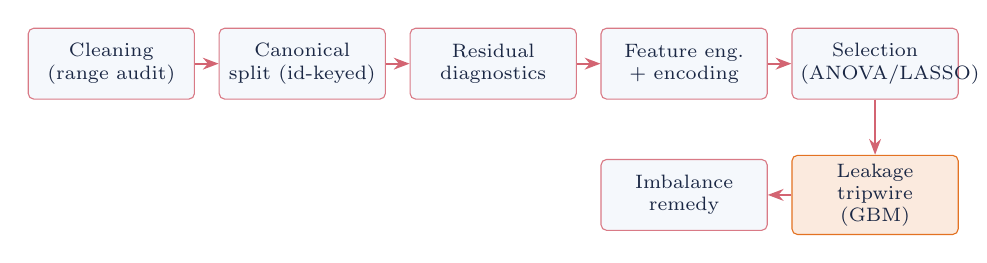
\begin{tikzpicture}[node distance=0.3cm]
    \node[pstep] (a) {Cleaning\\(range audit)};
    \node[pstep,right=of a] (b) {Canonical\\split (id-keyed)};
    \node[pstep,right=of b] (c) {Residual\\diagnostics};
    \node[pstep,right=of c] (d) {Feature eng.\\+ encoding};
    \node[pstep,right=of d] (e) {Selection\\(ANOVA/LASSO)};
    \draw[parrow](a)--(b);\draw[parrow](b)--(c);\draw[parrow](c)--(d);\draw[parrow](d)--(e);
    \node[pstep,below=0.7cm of e,fill=accent!15,draw=accent] (f) {Leakage\\tripwire (GBM)};
    \node[pstep,left=of f] (g) {Imbalance\\remedy};
    \draw[parrow](e)--(f);\draw[parrow](f)--(g);
  \end{tikzpicture}
  \end{center}
  \begin{columns}[T]
    \begin{column}{0.5\textwidth}
      \begin{block}{\small Cleaning result}
        \footnotesize 0 duplicates, 0 out-of-range rows --- the raw file was already clean. Cleaning is an \textbf{audited safety net}, not a fix.
      \end{block}
    \end{column}
    \begin{column}{0.5\textwidth}
      \begin{exampleblock}{\small Split discipline (fix vs.\ v1)}
        \footnotesize v1 split twice with two mechanisms. v2 uses \textbf{one} split (\texttt{split\_ids\_v2.json}), reused everywhere with \texttt{assert}.
      \end{exampleblock}
    \end{column}
  \end{columns}
\end{frame}

% ── Data prep: age non-linearity ──────────────────────────────────────────────
\begin{frame}{Churn is non-linear in age; \texttt{age\_band} wins on AIC (7387\(\to\)7063)}
  \aimtech{Diagnose and remediate the \texttt{age} non-linearity without leaking test data.}%
          {Pearson residuals from a logistic fit (train-only); \texttt{age\_band} vs.\ \texttt{age+age\(^2\)} compared by AIC.}
  \begin{columns}[T]
    \begin{column}{0.56\textwidth}
      \centering
      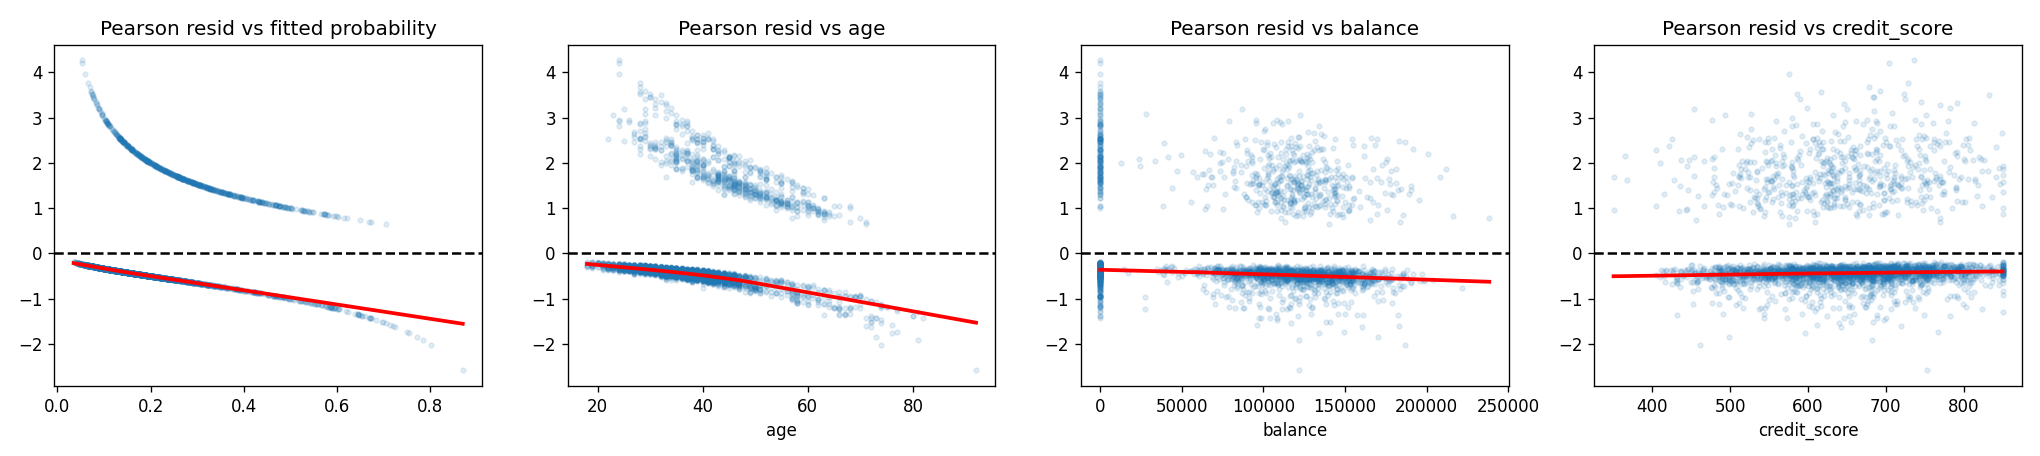
\includegraphics[height=0.32\textheight]{residual_diag_train_only_v2.png}\\[2pt]
      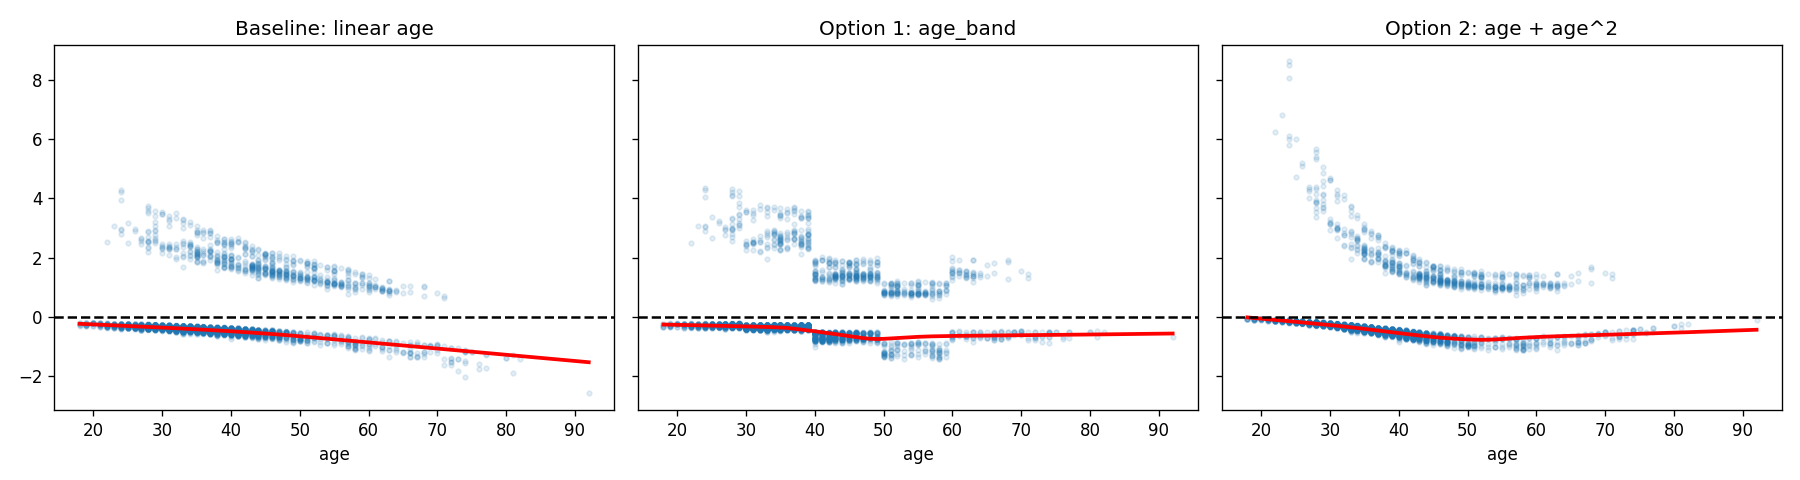
\includegraphics[height=0.30\textheight]{age_fix_comparison_v2.png}
    \end{column}
    \begin{column}{0.44\textwidth}
      \begin{insights}
        \begin{itemize}
          \item Binary target \(\to\) OLS residplot is the \textbf{wrong} diagnostic; use Pearson \((y-\hat p)/\sqrt{\hat p(1-\hat p)}\).
          \item AIC: linear 7387 \(\to\) \textbf{\texttt{age\_band} 7063} (winner) vs.\ \texttt{age+age\(^2\)} 7082.
          \item Both flatten the LOWESS trend; \texttt{age\_band} also communicates better (``risk peaks 50--59'').
          \item Decision rests on \textbf{8,000 train rows only} --- v1's leakage removed.
        \end{itemize}
      \end{insights}
    \end{column}
  \end{columns}
\end{frame}

% ── Data prep: leakage tripwire + imbalance ───────────────────────────────────
\begin{frame}{GBM leakage tripwire PASSES at 0.957\(<\)0.99 --- real-only signal is AUC 0.861}
  \aimtech{Prove the synthetic block cannot let a strong model ``cheat''.}%
          {Multivariate check with GradientBoosting on ALL / demo-only / behavioral-only feature sets.}
  \begin{columns}[T]
    \begin{column}{0.55\textwidth}
      \centering
      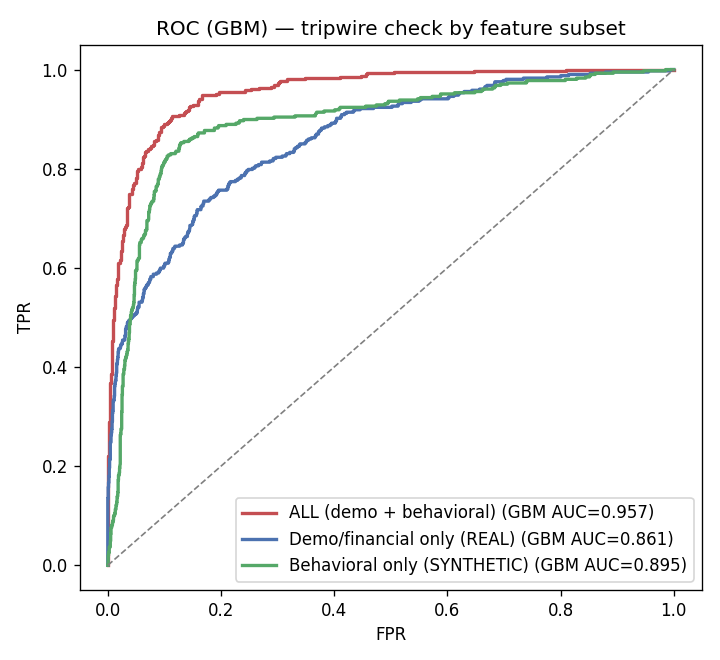
\includegraphics[height=0.66\textheight]{roc_leakage_check_v2.png}
    \end{column}
    \begin{column}{0.45\textwidth}
      \begin{insights}
        \begin{itemize}
          \item GBM (strongest class): max AUC-ROC \textbf{0.957 \(<\) 0.99 \(\to\) PASS}.
          \item \textbf{Demo-only (real): AUC-ROC 0.861 / PR 0.704} --- the only production-meaningful numbers.
          \item Behavioral-only 0.895 \(\to\) pipeline proof; the ALL gain is from the synthetic block.
        \end{itemize}
      \end{insights}
      \begin{block}{\small Imbalance decision}
        \footnotesize \texttt{class\_weight} \(\approx\) SMOTE (CV AUC-PR 0.804 vs.\ 0.802) \(\to\) pick \texttt{class\_weight}: simpler, no synthetic rows.
      \end{block}
    \end{column}
  \end{columns}
\end{frame}

% ═════════════════════════════════════════════════════════════════════════════
\section{Modeling \& Evaluation}
% ═════════════════════════════════════════════════════════════════════════════

% ── Modeling: champion model ──────────────────────────────────────────────────
\begin{frame}{Soft-voting ensemble on real features: AUC-ROC 0.861 [0.840--0.881]}
  \aimtech{Select a champion that is both strong and defensible under imbalance.}%
          {Logistic \(\to\) RandomForest / HistGBM \(\to\) soft Voting; 5-fold CV; permutation vs.\ impurity importance.}
  \begin{columns}[T]
    \begin{column}{0.55\textwidth}
      \centering
      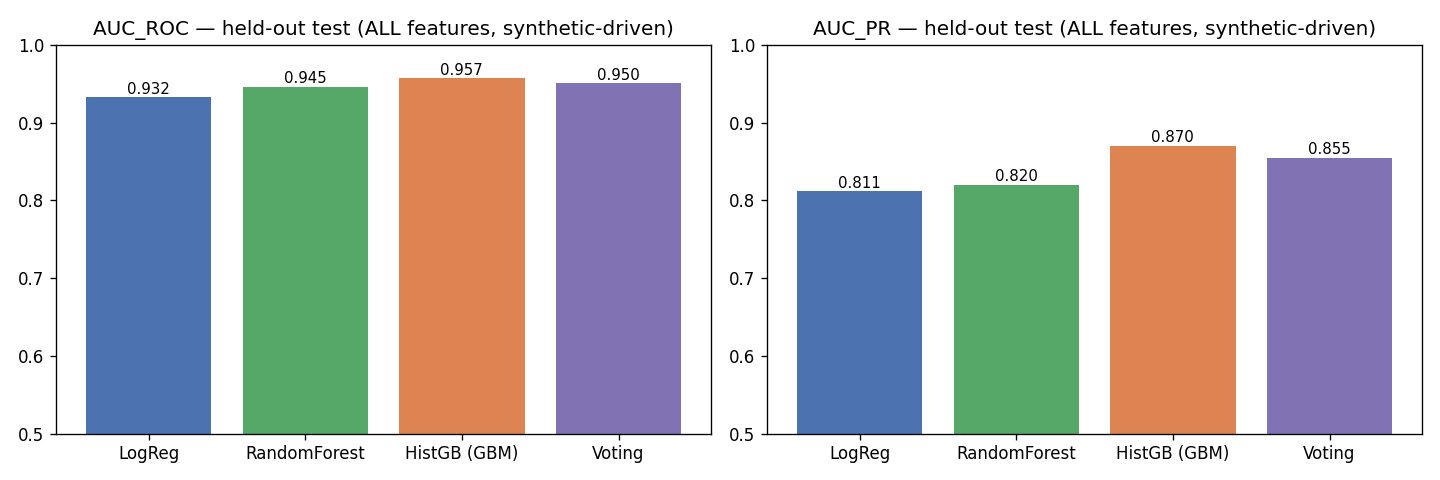
\includegraphics[height=0.33\textheight]{model_comparison_v2.png}\\[2pt]
      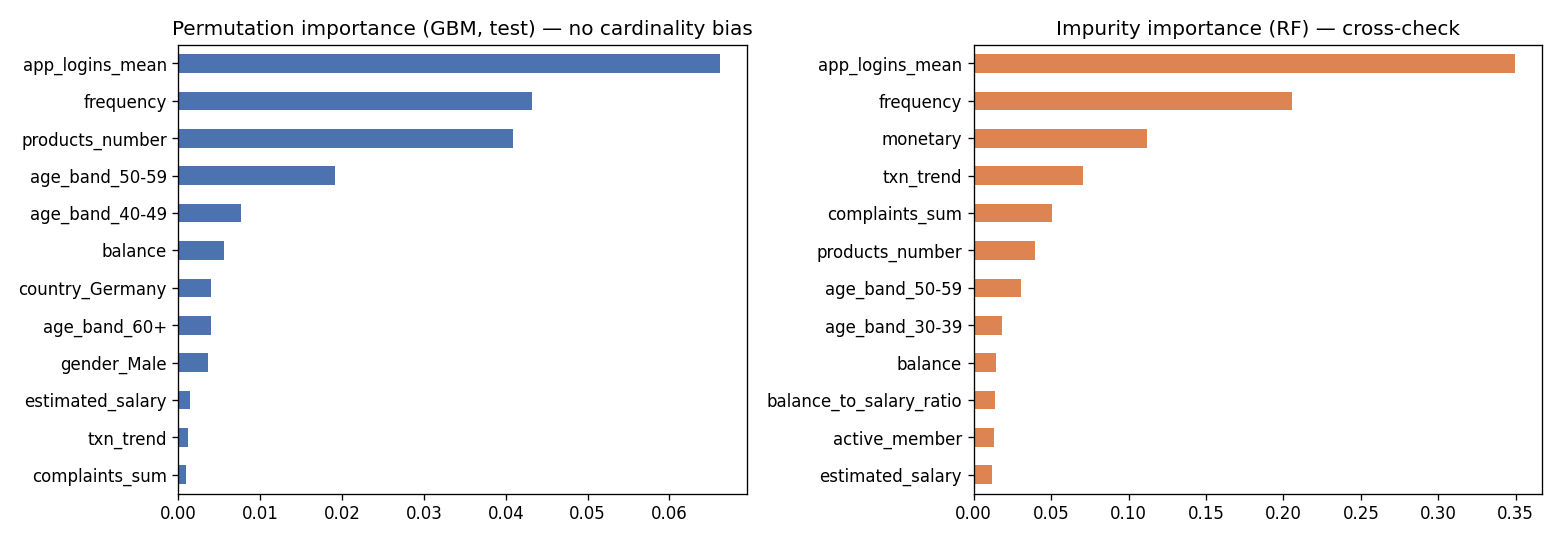
\includegraphics[height=0.29\textheight]{importance_comparison_v2.png}
    \end{column}
    \begin{column}{0.45\textwidth}
      \begin{insights}
        \begin{itemize}
          \item Champion chosen by \textbf{test AUC-PR} (right metric under 1:4 imbalance).
          \item Demo-only HistGBM: \textbf{AUC-ROC 0.861} [bootstrap 95\% CI 0.840--0.881], \textbf{AUC-PR 0.704}.
          \item Permutation \& impurity rankings \textbf{agree} on the top real drivers \(\to\) \texttt{products\_number}, \texttt{age\_band}, \texttt{active\_member}.
          \item ALL-feature ``importances'' are self-fulfilling (synthetic) --- reported but not interpreted.
        \end{itemize}
      \end{insights}
    \end{column}
  \end{columns}
\end{frame}

% ── Evaluation: budget-K operating point ──────────────────────────────────────
\begin{frame}{At a 10\% outreach budget: Precision@10 = 0.855, a 4.2\(\times\) lift}
  \aimtech{Turn a probability score into a retention decision under a fixed budget.}%
          {Precision@K / Recall@K vs.\ budget; calibration + Brier; bootstrap 95\% CI (500 resamples).}
  \begin{columns}[T]
    \begin{column}{0.55\textwidth}
      \centering
      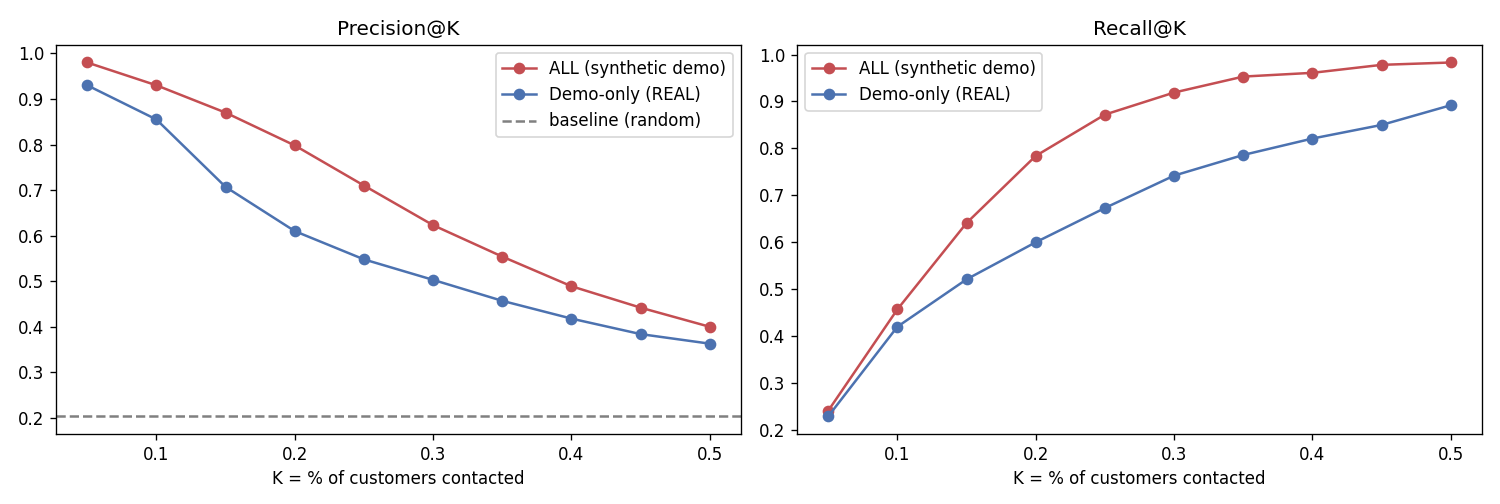
\includegraphics[height=0.34\textheight]{precision_recall_at_k_v2.png}\\[2pt]
      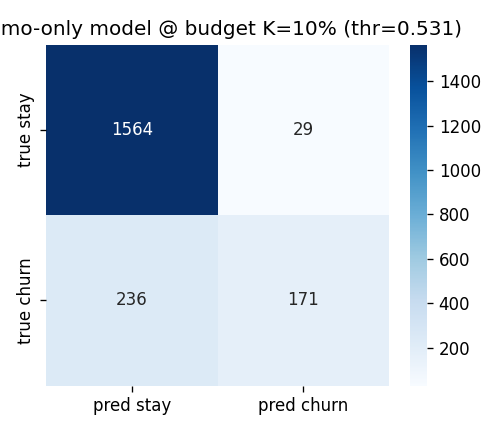
\includegraphics[height=0.24\textheight]{confusion_at_budget_v2.png}
    \end{column}
    \begin{column}{0.45\textwidth}
      \begin{insights}
        \begin{itemize}
          \item AUC is not an operating decision --- retention runs on a \textbf{budget of K\%}.
          \item At \textbf{K=10\%}: \textbf{Precision@10 = 0.855}, lift \textbf{4.2\(\times\)} over the 20.37\% base rate.
          \item Threshold = 90th percentile of scores; revisit against the \emph{actual} budget.
          \item Calibration checked (Brier) so probabilities can feed expected-value math.
        \end{itemize}
      \end{insights}
      \sowhat{Contact the top decile \(\to\) most churners at one-tenth the cost.}
    \end{column}
  \end{columns}
\end{frame}

% ═════════════════════════════════════════════════════════════════════════════
\section{Prediction System Deployment}
% ═════════════════════════════════════════════════════════════════════════════

% ── Deployment: pipeline + model card ─────────────────────────────────────────
\begin{frame}{Deployed as one reproducible \texttt{Pipeline} with a model card}
  \aimtech{Package the real-feature model so others can reproduce or challenge it.}%
          {sklearn \texttt{Pipeline} (preprocess+model) + JSON model card (metrics, features, seed, caveats).}
  \begin{columns}[T]
    \begin{column}{0.56\textwidth}
      \centering
      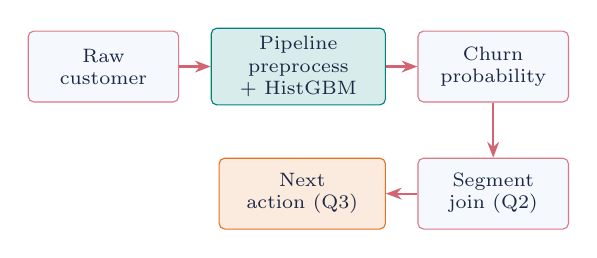
\begin{tikzpicture}[node distance=0.4cm]
        \node[pstep,text width=1.7cm] (r) {Raw\\customer};
        \node[pstep,text width=2.0cm,right=of r,fill=secondary!15,draw=secondary] (p) {Pipeline\\preprocess + HistGBM};
        \node[pstep,text width=1.7cm,right=of p] (s) {Churn\\probability};
        \node[pstep,text width=1.7cm,below=0.7cm of s] (g) {Segment\\join (Q2)};
        \node[pstep,text width=1.9cm,left=of g,fill=accent!15,draw=accent] (act) {Next\\action (Q3)};
        \draw[parrow](r)--(p);\draw[parrow](p)--(s);\draw[parrow](s)--(g);\draw[parrow](g)--(act);
      \end{tikzpicture}
    \end{column}
    \begin{column}{0.44\textwidth}
      \begin{block}{\small Model card (excerpt)}
        \footnotesize
        \begin{itemize}
          \item HistGradientBoosting, \textbf{real features only} (20).
          \item \texttt{seed=42}, \(n_{\text{train}}\)=8{,}000, \(n_{\text{test}}\)=2{,}000.
          \item Test: AUC-ROC \textbf{0.861}, AUC-PR \textbf{0.704}; budget K=10\%.
          \item Caveats: cross-sectional label; synthetic behavioral features \textbf{excluded}; uplift not causally validated.
        \end{itemize}
      \end{block}
    \end{column}
  \end{columns}
\end{frame}

% ── Inference: action mapping ─────────────────────────────────────────────────
\begin{frame}{Inference joins Q1 probability \(\times\) Q2 segment into a Q3 action}
  \aimtech{Make the score operational --- one row per customer, one recommended action.}%
          {Load saved pipeline \(\to\) score test customers \(\to\) join segment \(\to\) map to a playbook.}
  \renewcommand{\arraystretch}{1.3}
  \begin{center}
  \footnotesize
  \begin{tabularx}{\textwidth}{@{}p{0.22\textwidth}p{0.13\textwidth}p{0.10\textwidth}X@{}}
    \toprule
    \textbf{Segment} & \textbf{Churn rate} & \textbf{Score} & \textbf{Recommended next action} \\
    \midrule
    At Risk & 70\% & High & Priority win-back: human outreach + tailored offer (A/B-tested) \\
    Promising & mid & Med & Onboarding nudges to raise early activation \\
    Loyalist & mid & Low--Med & Cross-sell to the 2-product ``sweet spot'' \\
    Champion & 5.4\% & Low & Protect CLV: proactive perks, do \emph{not} discount \\
    \bottomrule
  \end{tabularx}
  \end{center}
  \begin{exampleblock}{\small From prediction to prescription}
    \footnotesize The system delivers a ranked top-K list \emph{plus} the segment context that decides \textbf{which} retention lever to pull --- not just a probability.
  \end{exampleblock}
\end{frame}

% ═════════════════════════════════════════════════════════════════════════════
\section{Open Questions \& Discussion}
% ═════════════════════════════════════════════════════════════════════════════

% ── Two-layer conclusions ─────────────────────────────────────────────────────
\begin{frame}{Conclusions are stratified: real-data insights vs.\ pipeline proof}
  \begin{columns}[T]
    \begin{column}{0.5\textwidth}
      \begin{exampleblock}{\small Layer A --- REAL data (business-safe)}
        \footnotesize
        \begin{itemize}
          \item \texttt{products\_number}\(\geq\)3 is the strongest red flag (4\(\to\)100\%, 3\(\to\)82.7\%) --- a no-model rule.
          \item Churn peaks at \textbf{56\%} for ages 50--59; \texttt{age\_band} beats raw age (AIC 7387\(\to\)7063).
          \item Segments: At Risk \textbf{70\%} (\(n\)=1,248) vs.\ Champion \textbf{5.4\%} (\(n\)=1,096).
          \item GBM demo-only: AUC-ROC \textbf{0.861}, Precision@10\% \textbf{0.855}, lift \textbf{4.2\(\times\)}.
        \end{itemize}
      \end{exampleblock}
    \end{column}
    \begin{column}{0.5\textwidth}
      \begin{alertblock}{\small Layer B --- PIPELINE only (synthetic)}
        \footnotesize
        \begin{itemize}
          \item Generator v3 keeps signal learnable (0.895) yet below the 0.99 tripwire even for GBM (max 0.957).
          \item Full chain runs end to end, reproducibly (seed 42, model card).
          \item ``Top'' behavioral features are self-fulfilling by construction --- they prove the \emph{code}, not the world.
        \end{itemize}
      \end{alertblock}
    \end{column}
  \end{columns}
  \sowhat{We publish externally \emph{only} Layer A; Layer B documents that the machinery is trustworthy.}
\end{frame}

% ── Next steps / open questions ───────────────────────────────────────────────
\begin{frame}{Open questions \& next steps}
  \begin{columns}[T]
    \begin{column}{0.5\textwidth}
      \begin{block}{\small Limitations}
        \footnotesize
        \begin{itemize}
          \item Churn label is \textbf{cross-sectional} (no timestamp) --- a 90-day window would relabel some customers.
          \item Behavioral evidence is \textbf{synthetic}; trend claims await real transaction history.
          \item Retention uplift is \textbf{assumed}, not measured.
        \end{itemize}
      \end{block}
    \end{column}
    \begin{column}{0.5\textwidth}
      \begin{exampleblock}{\small Next steps}
        \footnotesize
        \begin{enumerate}
          \item Swap synthetic tables for real transactions; redefine churn over 90 days; rerun from Data Prep §7.
          \item \textbf{A/B test} the At-Risk offer to measure true uplift (replaces the 30\% assumption).
          \item Add \texttt{CalibratedClassifierCV} if probabilities feed expected value.
          \item Monitor PSI/drift + AUC by monthly cohort in production.
        \end{enumerate}
      \end{exampleblock}
    \end{column}
  \end{columns}
  \sowhat{The only way to claim causal churn reduction is a live A/B test --- everything above is observation \& prediction.}
\end{frame}

% ── THANK YOU ─────────────────────────────────────────────────────────────────
\begin{frame}[noframenumbering]{}
  \begin{center}
    \vspace{0.8cm}
    {\huge \textbf{Thank You}}\\[0.4cm]
    {\large Questions \& Discussion}\\[0.8cm]
    \rule{0.65\textwidth}{0.4pt}\\[0.3cm]
    {\footnotesize Customer Churn Prediction \& Segmentation for a Digital Bank --- SOICT, HUST}
  \end{center}
\end{frame}

\end{document}
